%!TEX root = ../report.tex

\begin{document}
    \chapter{Methodology}

    How you are planning to test/compare/evaluate your research.
    Criteria used.

    \section{Introduction}

    \section{Structure of the chapter}
    This chapter aims to explain the two state-of-the-art uncertainty estimation methods compared in this research work. The sections \ref{general_framework} and \ref{der} give an intuitive explanation of the methods.
    
    \section{A General Framework for Uncertainty Estimation in Deep Learning}\label{general_framework}
    \subsection{Overview}\label{mcdo_adf_overview}
    This work proposes a technique to distinctively estimate data and model uncertainties associated with an output of any Neural Network model.The technique is here after referred to as "MCDO\_ADF", representing the fact that is a combination of two ideas, Monte-Carlo Drop Out(MCDO) and Assumed-Density-Filtering (ADF). MCDO\_ADF treat the  two uncertainty components to be related, which sets it apart from most of other uncertainty estimation methods that treat them to be independent. The method employs Bayesian Belief Networks combined with Monte-Carlo sampling for estimating the model uncertainty and relies on the idea of Assumed Density Filtering for  estimating data uncertainty associated with an output. 
    
    Authors of the MCDO\_ADF technique claim it to be a general framework to estimate uncertainties in Neural Networks. They give following reasons to validate their claim:
    \begin{itemize}
    	\item Using this uncertainty estimation method does not require any architectural changes in the target Neural Network.
    	\item Applicability of the method to Neural Network models of different tasks.
    	\item Absence of any need of make changes in the optimization process.
    	\item Ability of the technique to be applied to already trained models.
    \end{itemize}
	
	The upcoming sections of this chapter explain the MCDO\_ADF technique  and also analyze its claimed "generality" by using it in a Resnet8 based Neural Network regression model meant for the application of steering-angle prediction in autonomous cars.(Note: A detailed description of the data set, training and inference procedures of the Neural Network model is available in the next chapter[]).  
	
	
    \subsection{Integrating MCDO\_ADF with a Neural Network and estimating uncertainties}
    \subsubsection{MCDO\_ADF as an algorithm}
    Estimating uncertainty using the MCDO can be formulated as an algorithm consisting of the following steps:
    \begin{itemize}
    	\item Transform the Neural Network of interest to its ADF(Assumed Density Filtering) version.
    	\item Collect a predefined number(T) of Monte-Carlo(MC) samples by forwarding inputs and noise variances $(x,v))$ stochastically through the network for T times.
    	\item Computation of output predictions and uncertainties  
    \end{itemize}
	\begin{figure}[h]
	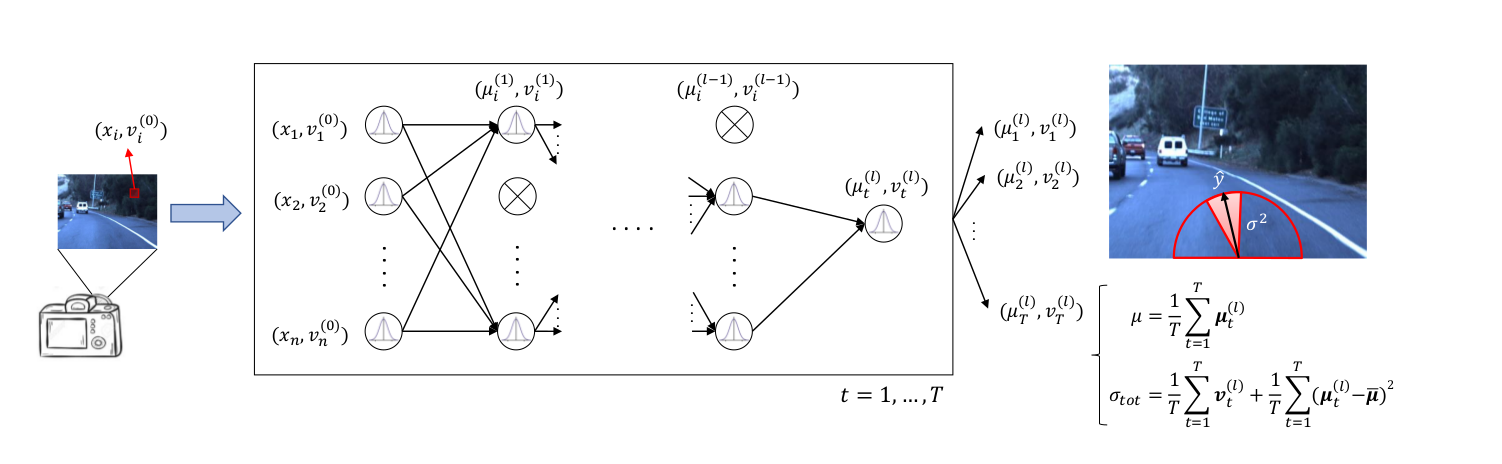
\includegraphics[scale=0.35]{adf_mcdo}
	
	\caption{Illustration of the MCDO\_ADF technique.Here $x_{i}$ denotes the input through the $i^{th}$ unit of a given hidden layer,$x_{i^{(n)}}$ denotes the noise variance input to the ith unit of the nth layer. Circles with crosses inscribed denote the dropped out neurons whereas the ones with the Gaussian distribution symbol denote the active units. T values of $\mu$ and $v$ are collected from T stochastic forward passes. Image source: }
	\label{fig_adf_mcdo}
	\end{figure}





	\subsubsection{Assumed Density Filtering (ADF)}
	The MCDO\_ADF technique considers sensor noise to be the primary source of data uncertainty in neural network predictions and therefore feeds it to the Neural Network model during the inference. In order to propagate the input data distribution (parameterized by the input as its mean and sensor noise as variance) the technique of ADF is used. Briefly in the context of MCDO\_ADF, ADF replaces every input activation into a probability distribution and also approximates the same using a tractable Gaussian distribution and makes both the mean and noise variance available in the output layer.Following points describe Assume Density Filtering in a more detailed manner:
	\begin{itemize}
		\item Assumed Density Filtering(ADF) is a technique in Bayesian machine learning to approximate intractable and complex distribution with distributions that are easy to handle. In the case of Bayesian Inference, ADF aims to project the true posterior onto a distribution of choice. The exponential family of distributions are a popular choice.
		\item In the case of MCDO\_ADF there is a need to propagate the input data distribution so that the values of its mean and variance (noise variance) are available in the output layer. 
		\item The input data distribution is considered to be Gaussian in nature. Every intermediate layer outputs the transformed version of the input distribution.  However, when it propagates through non-linearities in a Neural Network the resulting distribution need not be essentially another Gaussian. Such a distribution emerging out of non-linear blocks is also conditioned by distribution over activations of the preceeding layers. Therefore, the resulting distribution becomes intractable.
		\item Such intractable and complex distributions are estimated using ADF by:
		\begin{itemize}
			\item Assuming conditional independence between distribution outputted from a given layer with its preceeding layers. 
			\item Approximating the complex distribution with a Gaussian distribution whose pair has the least possible value of Kullback-Leibler divergence([]). ADF achieves this by matching the first two moments of the distributions.
			\item In practice, this is achieved by optimizing the global variational objective([]).
		\end{itemize} 
	\end{itemize}
	In practice, every building block of a Neural Network has its corresponding ADF version and therefore during the inference time the entire model has to be transformed to its ADF equivalent. This gives the ability to the Neural Network model to propagate and output distributions which represent data uncertainty.
	\begin{figure}[h]
		\centering
		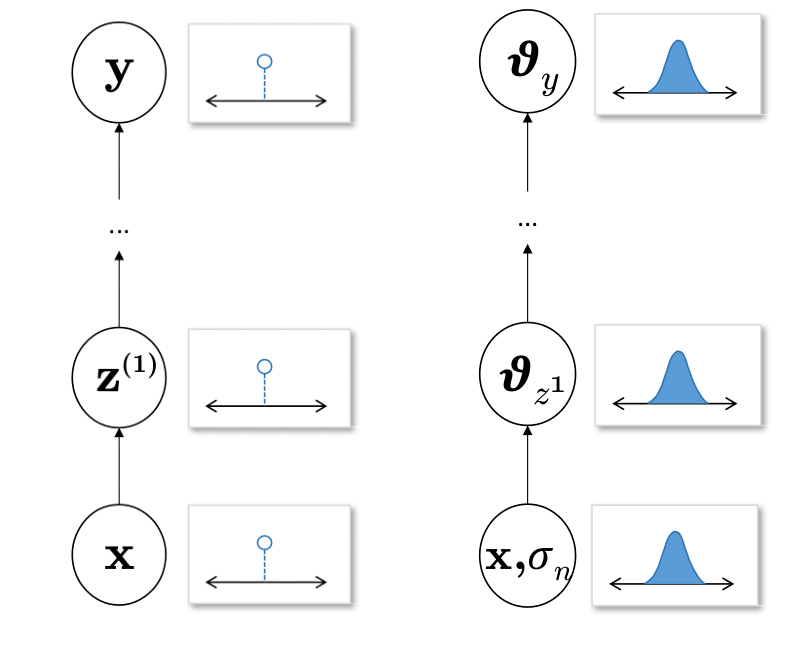
\includegraphics[scale=0.4]{adf_determ}
		\caption{Illustration of forward passes in deterministic and ADF versions of a Neural Network. Here $x$ denotes the input activations,$z^(n)$ denotes activation input to the nth layer,$y$ denotes the output, $\theta_{z^n}$ represents input activation to the nth layer expressed as a probability distribution and $\sigma$ corresponds to the noise variance. Image source: }
	\end{figure}
		
	\subsubsection{Data uncertainty estimation}
	The ADF transformed Neural Network produces two outputs from the final layer: mean ($\mu_{t^{(l)}}$) and variance($v_{t^{(l)}}$ of the propagated distribution, as shown in the figure \ref{fig_adf_mcdo}. The pair of values is outputted for each of the T stochastic forward passes (described in the next paragraph) and the mean of T variance values is considered to be the value of data uncertainty. Likewise, the mean of T predictions is considered to be the model's prediction for the given input.
	\begin{equation}
	prediction = \mu = \frac{1}{T}\sum_{t=1}^{T}\mu_{t^{(l)}}
	\end{equation}	 
	\begin{equation}
		data\_uncertainty = \sigma_{data}=\frac{1}{T}\sum_{t=1}^{T}v_{t^{(l)}}
	\end{equation}

	\subsubsection{Monte-Carlo Dropout (MCDO)}
	
	This uncertainty estimation method relies on the idea of Monte-Carlo(MC) sampling to estimate model uncertainty associated any prediction. In practice, MC sampling is achieved by enabling dropout during the test time and obtaining the desired number of samples (T), which are nothing but outputs of the Neural Network model during different forward passes of the input. Enabling dropout introduces stochasticity during those forward passes.
	
	Following points briefly describe the dropout technique in a general context:
	\begin{itemize}
		\item Dropout([]) is primarily a regularization technique used while training Neural Networks in order to avoid over-fitting.
		\item During dropout certain nodes of a given Neural Network layer are not considered for training. The nodes are ignored with a probability equal to the dropout rate (often denoted by $\textbf{p}$).
		\item Using dropout during training makes Neural Network layers to adapt in such a way that they cope with mistakes made my the prior layers. 
		
	\end{itemize}
	 
	In the context of Bayesian inference, the Dropout technique is used to approximate the posterior distribution over weights of a given Neural Network, when the training data and labels are given ($P(W|X,Y))$. The approximation is obtained by applying dropout at the test-time. This makes it possible to obtain multiple predictions for any given input from different architectures resulting from application of dropout to the base Neural Network model. The different architectures obtained along with their weights can be considered as Monte-Carlo(MC) samples from the space of all possible architectures. The number of MC samples to be obtained is a hyper-parameter and denoted by $T$. In another perspective, $T$ equals the number of forward passes through different architectures with different sets of weights $\{W_{1}^t,..,W_{L}^t\}_{t=1}^T$($L$ denotes the number of dropout applied layers in the Neural Network). The first and second moments (mean and variance) of predictions obtained from these stochastic forward passes of given input are utilized to compute model uncertainty(explained in  \ref{adf_mcdo_uncertainty_estimation}). One of the highlights of this technique is that its usage does not require any architectural changes and also can applied to already trained Neural Net models. The hyper-parameters $T$ and $p$ significantly impact the effectiveness of this technique. In the case of $p$ a very high value (close to 1) increases sparsity in nodes and also results in longer convergence-time while a low value eliminates the MC-sampling utility. For our experiment, the value of $p=0.02$ is used. The hyper-parameter $T$ significantly impacts the inference time of a Neural Network model and therefore has to be chosen optimally based on the run-time requirement of the system where the model would be deployed.

	\subsubsection{Model uncertainty estimation}
 	The MCDO\_ADF technique estimates model uncertainty using predictions generated from the Neural Network model during multiple(T) forward passes, while the dropout is enabled. A given input is processed by the model T times, with a new combination of neurons considered for almost every forward pass. This produces an effect of gathering predictions from an ensemble consisting of T Neural Net models with different architectures. The variance of T gathered predictions is the estimated model uncertainty. In the following equations $\mu_{t^{(l)}}$ signifies the mean output from the ADF transformed version of the Model during $t^{th}$ forward pass.
 	
 	\begin{equation}
 		model\_uncertainty = \sigma_{model} =  \frac{1}{T}\sum_{t=1}^{T}(\mu_{t^{(l)}}-\overline{\mu})^2
 	\end{equation}
 	\begin{equation} 
		where, \overline{\mu} = \frac{1}{T}\sum_{t=1}^{T}(\mu_{t^{(l)}} 
	\end{equation}
	\subsubsection{Combining ADF and MCDO}
	The MCDO\_ADF method considers a relationship to exist between the two components of uncertainty (data and model). The relationship  is realized in this technique by combining both the ideas of ADF and MCDO. During inference,  
	\begin{itemize}
		\item The given Neural Network model is transformed to its ADF equivalent so that the output layer produces both predictions(mean) and noise variance as the model's final outputs.
		\item For estimating model uncertainty,  dropout is enabled in the ADF transformed version of the original Neural Network following which T MC samples are collected during T stochastic forward passes. It is this application of dropout on the ADF transformed version that produces the "effect of ensembling T ADF Neural Networks" and also considers any relationship between the two uncertainty components.
		\item Combining ADF and MCDO leads to another intuitive realization about the uncertainty components in this setup. Even when a particular input fed to the Neural Net model was observed frequently during training, if corrupted due to sensor noise then it will not only have high values of both data and model uncertainties. 
		
	\end{itemize}
    
    \subsubsection{Total uncertainty}
    The predictive uncertainty is estimated by summing up both its components (data and model) and is given by the following equation.
    \begin{equation}
    	predictive\_uncertainty = \sigma_{total} =  \frac{1}{T}\sum_{t=1}^{T}((\mu_{t^{(l)}}-\overline{\mu})^2 + v_{t^{(l)}})
    \end{equation}
    

    In summary, both ADF and MCDO techniques approximate probability distributions of data and model with Normal distributions respectively. ADF propagates the input data distribution and approximates them as Gaussians in every Neural Network layer while MCDO approximates the distribution around weights by sampling and forms a Gaussian distribution out of the samples. The variances of these Gaussian distributions are considered to be the uncertainty components and are summed up to yield the predictive uncertainty.
    
    \subsection{Inference procedure}
    The MCDO\_ADF method can be applied to already trained deterministic version of the Neural Network models as mentioned in \ref{mcdo_adf_overview}. However, it is also possible to train the Neural Network model of interest with dropout enabled and use the same for inference.
    In order to estimate the predictive uncertainty during inference:
    \begin{itemize}
    	\item Every layer of the Neural Network has to replaced with its ADF equivalent so that they are equipped with the ability to propagate data distributions. The implementation of ADF equivalents for most of the Neural Network building blocks is available in [].
    	\item The value of noise variance (a constant value) obtained from the sensor's data sheet is fed along with the input data to the ADF transformed input layer of the network. During propagation through intermediate layers, it is ensured that at least a minimum value of variance is propagated. In the case of experiment described in the next chapter, a minimum value of 0.001 is used.
    	\item Every input along with the noise variance undergoes T stochastic forward passes through the network to generate T predictions.  
    \end{itemize}
     The experiment described in the next chapter discusses more on practical aspects of this technique.    
    \subsection{Downsides}
    \begin{itemize}
    \item The need for multiple (T) forward passes to obtain MC samples is computationally expensive and cannot be afforded in the case of real-time systems.While there is an option to reduce the value of T, it increases the difference between approximated and underlying distribution over weights of the model, thereby affecting the method's performance. 
    \item The method considers sensor noise to be the only source of data uncertainty. Also, it treats the noise to be additive Gaussian in nature. However, sensor noise is just one of the factors contributing to data uncertainty. For instance, in the case of image data, usage of a lossy compression technique can also contribute to its noise. Also, it is possible for a given sensor to produce data whose noise levels differ. As it is impossible to consider and model every possible noise source, it is important for an uncertainty estimation method to learn to differentiate noise and useful information from given data.
    \item The authors of MCDO\_ADF quote its ability to be applied to already trained models as one of the key reasons for its generality. However, retraining a Neural Network model is something feasible in most of the cases.
    \item As hyper parameters such as drop-out rate($p$), number of MC samples(T) and noise variance have a major role to play in this technique, it adds to the responsibilities of the practitioner to optimally choose them based on the problem at hand.
	    \end{itemize}    
    **Downsides of MCDO and ADF to be read and listed**\pagebreak
    \section{Deep Evidential Regression}\label{der}
\end{document}
